\documentclass[11pt]{article}
\usepackage{amsmath,amssymb,amsthm}
\usepackage{graphicx,booktabs,hyperref}

% text and math macros
\newcommand{\term}[1]{\emph{#1}}
\newcommand{\abs}[1]{\left|#1\right|}
\newcommand{\R}{\mathbb{R}}
\DeclareMathOperator{\tr}{tr}
\newcommand{\be}{\begin{equation}}
\newcommand{\ee}{\end{equation}}

\newtheorem{theorem}{Theorem}[section]
\newtheorem{lemma}[theorem]{Lemma}
\theoremstyle{definition}
\newtheorem{definition}[theorem]{Definition}
\theoremstyle{remark}
\newtheorem*{remark}{Remark}

\title{A sample document for \texttt{latex2mobile}\thanks{This file exercises most supported features.}}
\author{Ada Example \and Bo Tester}
\date{September 2026}

\begin{document}
\maketitle

\begin{abstract}
We collect the constructs that \texttt{latex2mobile} converts: numbered equations and
alignments, theorem-like environments in three styles, lists, tables, figures,
footnotes and citations~\cite{Dyson:1962,Mehta:2004}.
\end{abstract}

\section{Introduction}
\label{sec:intro}

Random matrices appear everywhere~\cite{Altland:1997}. A \term{Wigner matrix} $H=H^\dagger$ has
eigenvalue density that approaches the semicircle,\footnote{For the Gaussian ensemble with the
normalization of~\eqref{eq:gauss}.}
\be
\rho(E)=\frac{1}{2\pi}\sqrt{4-E^2},\qquad \abs{E}\le 2 .
\label{eq:semicircle}
\ee
The Gaussian weight is
\begin{equation}
P(H)\,dH\propto e^{-\frac{N}{4}\tr H^2}\,dH, \qquad H\in\R^{N\times N}.
\label{eq:gauss}
\end{equation}
Quotes ``like this'', an en dash 1--2, an em dash---and accents: Schr\"odinger, Poincar\'e, Erd\H{o}s.
Inline math also works with \(x\in\R\).

\subsection{Alignments}
Numbered rows, an unnumbered row, and a split equation:
\begin{align}
  a &= b + c \label{eq:first}\\
  d &= e + f + g \nonumber\\
  h &= \int_0^1 x^2\,dx = \frac13 \label{eq:third}
\end{align}
\begin{equation}
\begin{split}
  (a+b)^2 &= a^2 + 2ab + b^2\\
          &\ge 4ab .
\end{split}
\label{eq:split}
\end{equation}
Equations \eqref{eq:first} and \eqref{eq:third} are rows of one alignment, and~\eqref{eq:split} is a split.
\begin{multline}
  f(x) = a_0 + a_1 x + a_2 x^2 + a_3 x^3 + a_4 x^4 \\
  + a_5 x^5 + a_6 x^6 + a_7 x^7 .
\end{multline}
\[
  \sum_{n=1}^\infty \frac{1}{n^2} = \frac{\pi^2}{6}
\]

\section{Results}
\label{sec:results}

\begin{definition}[Semicircle law]
\label{def:sc}
A sequence of ensembles obeys the \emph{semicircle law} if its density converges to~\eqref{eq:semicircle}.
\end{definition}

\begin{theorem}[Wigner]
\label{thm:wigner}
Wigner matrices obey the semicircle law (Definition~\ref{def:sc}).
\end{theorem}

\begin{lemma}
\label{lem:moments}
The even moments of the semicircle are the Catalan numbers $C_k=\frac{1}{k+1}\binom{2k}{k}$.
\end{lemma}

\begin{proof}[Proof of Lemma~\ref{lem:moments}]
Count non-crossing pairings. Then apply Theorem~\ref{thm:wigner}.
\end{proof}

\begin{remark}
Unnumbered remarks use the remark style.
\end{remark}

\subsection{Lists}
\begin{itemize}
  \item a bullet with math $E_0>0$;
  \item a bullet with a nested list:
  \begin{enumerate}
    \item first;
    \item second.
  \end{enumerate}
  \item[$\star$] a custom label.
\end{itemize}
\begin{description}
  \item[GOE] real symmetric matrices;
  \item[GUE] complex Hermitian matrices.
\end{description}

\subsection{Tables and figures}
Table~\ref{tab:dyson} lists Dyson's three classes, and Figure~\ref{fig:edge} shows a soft edge.
\begin{table}[h]
\centering
\caption{The threefold way.}
\label{tab:dyson}
\begin{tabular}{lcr}
\toprule
ensemble & $\beta$ & symmetry \\
\midrule
GOE & 1 & time reversal, $T^2=1$ \\
GUE & 2 & none \\
GSE & 4 & time reversal, $T^2=-1$ \\
\midrule
\multicolumn{3}{c}{Dyson (1962)} \\
\bottomrule
\end{tabular}
\end{table}

\begin{figure}[h]
\centering
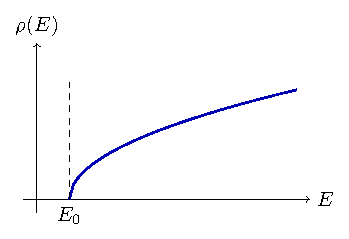
\includegraphics[width=0.7\textwidth]{figure}
\caption{A square-root edge at $E_0$.}
\label{fig:edge}
\end{figure}

\begin{quote}
A quotation, with a \verb|\verb| command and a URL: \url{https://arxiv.org}.
\end{quote}
\begin{verbatim}
python3 latex2mobile.py sample.tex
\end{verbatim}

\section*{Acknowledgments}
Thanks to \href{https://www.mathjax.org}{MathJax}.

\appendix
\section{An appendix}
\label{app:a}
Appendix equations are numbered by letter:
\begin{equation}
e^{i\pi}+1=0 .
\label{eq:euler}
\end{equation}
See~\eqref{eq:euler} and Section~\ref{sec:intro}.

\bibliographystyle{plain}
\bibliography{sample}
\end{document}
